\documentclass[11pt,a4paper]{article}
\usepackage[margin=1in]{geometry}
\usepackage{amsmath,amssymb,bm}
\usepackage{graphicx}
\usepackage{booktabs}
\usepackage{hyperref}

\title{Three-layer erf networks: a matrix mean-field theory and its test against the exact posterior}
\author{Akiva Lipshitz}
\date{9 November 2026}

\newcommand{\E}{\mathbb{E}}
\newcommand{\erf}{\operatorname{erf}}
\newcommand{\He}{\mathrm{He}}
\graphicspath{{../milestones/fcn3_collapsed_hmc/plots/ray/}{../milestones/fcn2_collapsed_hmc/figures/}}

\begin{document}
\maketitle

This week I completed a mean-field theory for the Bayesian posterior of a three-layer erf network and tested it, together
with the two-layer theory, against samples from the exact posterior. The two-layer theory becomes exact as the input
dimension grows along a ray of fixed theory parameters. For the three-layer network the learnabilities converge to the
theory in the same limit, once the substantial variation between training sets is averaged out and provided the hidden
width grows with $d$. The preactivations of the hidden layer are far from Gaussian, and the theory reproduces their
distribution at large $d$. In the read-in layer the inner well agrees with the theory, the excess of neurons between the wells
at $d=150$ is a finite-training-set effect, and with the theory's number of outer neurons the outer well's minimum lies
3\% inside the theory's at $d=300$ and 1\% inside at $d=600$; the number of read-in neurons in the outer well is not
equilibrated by the sampler, and its equilibrium distribution remains open. Intermediate steps of the derivation omitted here are given in
\texttt{notes/fcn3\_matrix\_eos.tex}.

%% =====================================================================
\section{Two-layer network}
%% =====================================================================
The two-layer theory is tested along the $\kappa_0=0.015$ ray, $N=1500$, $P=3000(d/150)^2$, $\kappa=0.015\,d/150$,
$\sigma_A^2=(8/1500)(150/d)$, on which the theory's parameters do not change with $d$; any remaining $d$-dependence of the
gap between theory and sampler measures what the theory leaves out. The sampler draws from the exact posterior on a
fixed training set, with the readout integrated out analytically, HMC on the remaining weights and exact per-neuron
jump moves. The three-layer network is tested on the same ray with a sampler built the same way.

The theory, with the perpendicular norm $q$ treated as a per-neuron variable and the $x_0$
tower taken to He$_{11}$, approaches the exact posterior steadily (table below, Figure~\ref{fig:fcn2}). At $d=600$--$1200$
it reproduces $L_3$ to within 0.4\% and $\langle w_0^2\rangle$ to within 0.2--1.5\%. Both corrections are needed: with $q$
frozen at its prior value, or with the tower stopped at He$_3$, the error in $L_3$ is 15--17\% and does not shrink with
$d$. At $d=75$, where $P=750<N$, the training set is too small to resemble the population and the theory fails.
\begin{center}
\begin{tabular}{@{}rccc@{}}
\toprule
$d$ & $\langle w_0^2\rangle$, HMC / theory & $L_3$, HMC / theory & raw gap (nats), HMC / theory\\
\midrule
75   & 0.0381 / 0.0429 & 0.318 / 0.391 & 4.11 / 3.91\\
150  & 0.0382 / 0.0388 & 0.370 / 0.387 & 3.95 / 3.94\\
300  & 0.0360 / 0.0367 & 0.376 / 0.385 & 3.97 / 3.96\\
600  & 0.0354 / 0.0356 & 0.381 / 0.383 & 3.96 / 3.96\\
800  & 0.0353 / 0.0353 & 0.382 / 0.382 & 3.92 / 3.97\\
1200 & 0.0345 / 0.0350 & 0.382 / 0.382 & 3.95 / 3.97\\
\bottomrule
\end{tabular}
\end{center}

The read-in action $-\log p(w_0)$ has an inner well at $w_0=0$ and an outer well at $|w_0|\approx1.2$, the outer one
holding the roughly 4\% of neurons aligned with the target. Every term of the action is of order $d$, so
$-\log p(w_0)=\beta\hat S(w_0)+O(1)$ with a $d$-independent leading part $\hat S_\infty$. If the two wells of
$\hat S_\infty$ differed in depth by $\delta$, the raw gap $\Delta=-\log p(w_{\rm out})+\log p(0)$ would grow as $\beta\delta$
and the aligned fraction would go to zero or one exponentially in $d$; a finite aligned fraction therefore requires
$\delta=0$, so that the wells are degenerate at leading order and only an $O(1)$ gap remains. The sampler confirms this:
over an eightfold range of $d$ its raw gap stays between 3.92 and 3.97 nats, where a non-degenerate action would have
taken it from about 4 to 32 nats (Figure~\ref{fig:gap}), and it agrees with the theory's gap to about 1\%. The
theory's subleading prediction $\Delta\simeq3.97-4.7/d$ is not resolved: it spans 0.06 nats over the whole range, which
is comparable to the scatter of the sampler, and $d=800$ lies about $3\sigma$ below it.

\begin{figure}[!htbp]
  \centering
  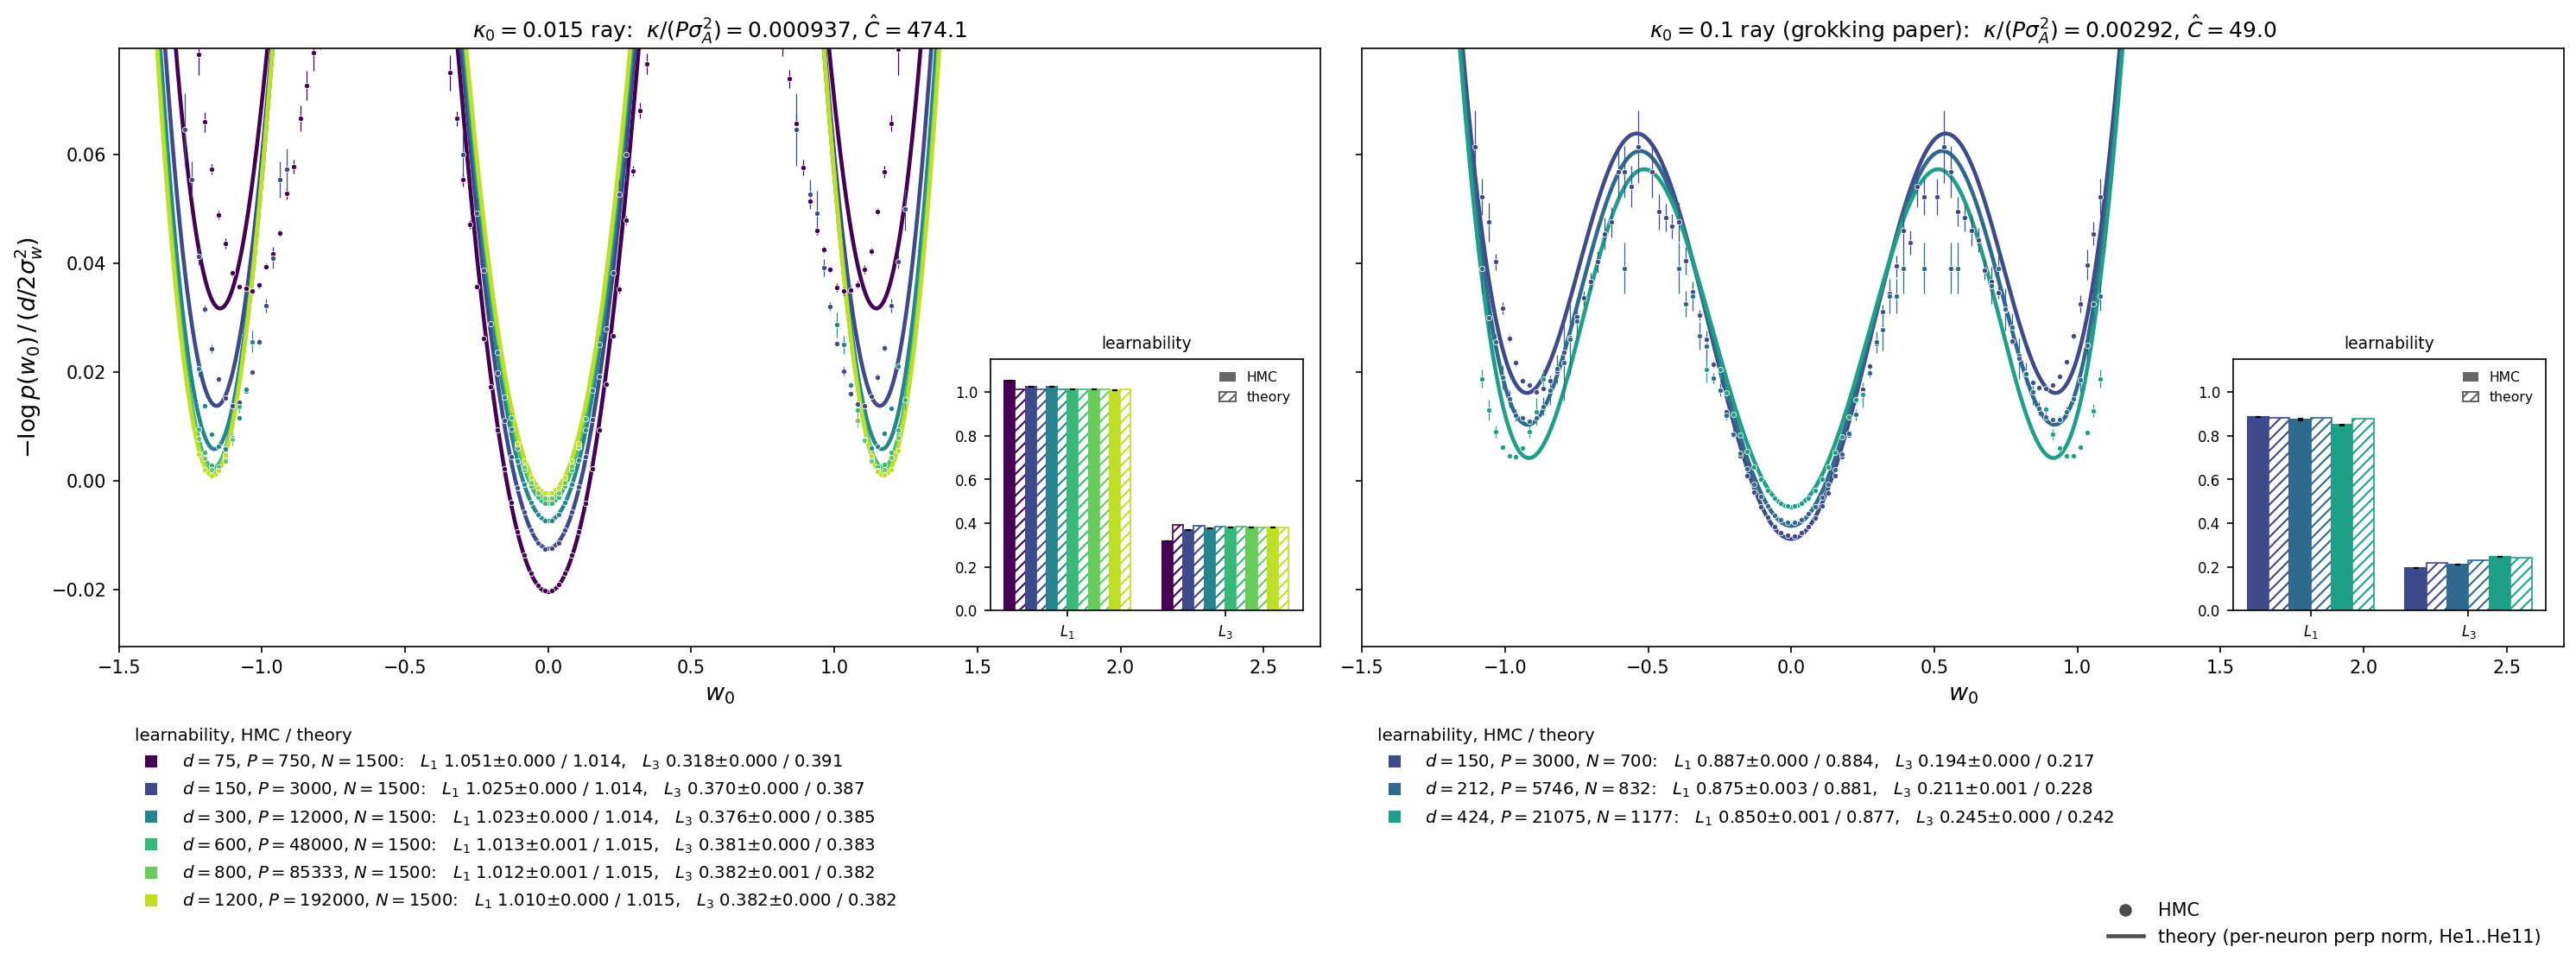
\includegraphics[width=\textwidth]{large_d_actions.png}
  \caption{Read-in action of the two-layer network, $-\log p(w_0)/\beta$, from theory (lines) and the exact sampler
  (points), with learnabilities in the insets. Left: $\kappa_0=0.015$ ray, $d=75$--$1200$. Right: $\kappa_0=0.1$ ray.}
  \label{fig:fcn2}
\end{figure}

\begin{figure}[!htbp]
  \centering
  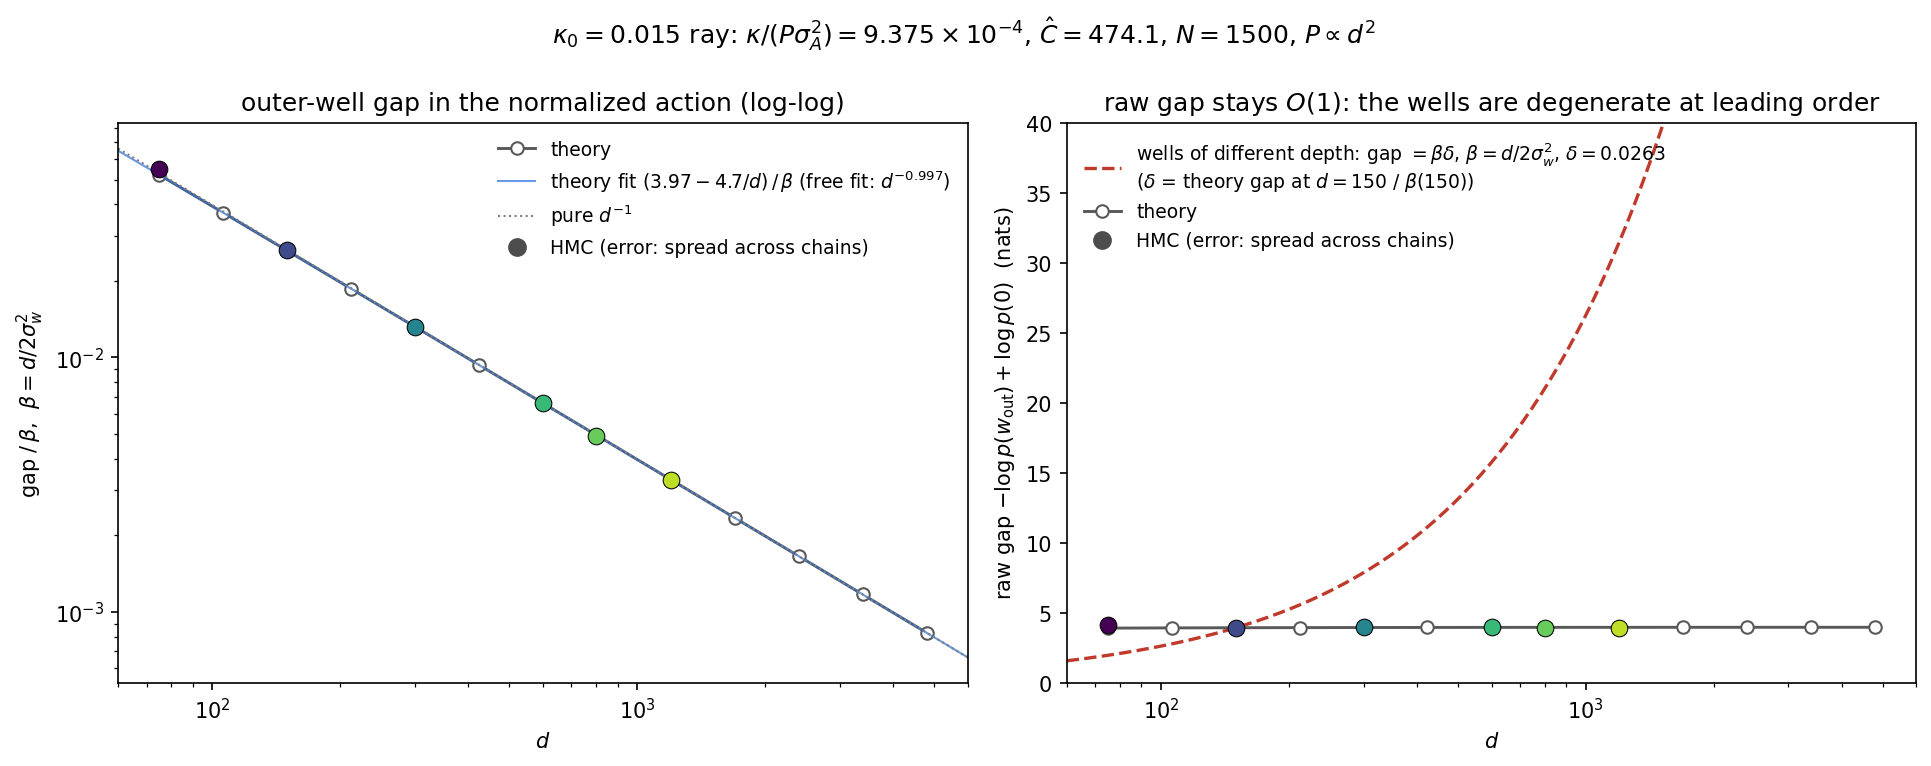
\includegraphics[width=\textwidth]{gap_scaling.png}
  \caption{Gap between the outer and inner wells of the two-layer read-in action. Left: normalised by $\beta$; the slope
  of $-1$ means the raw gap does not grow with $d$. Right: the raw gap against $d$. The dashed red line is the growth that wells of
  different depth at leading order would produce, $\Delta(d)=\beta\delta$ with $\beta=d/2\sigma_w^2=d$ and a $d$-independent
  depth difference $\delta$, here fixed by the theory's gap at $d=150$: $\delta=3.94/150=0.0263$, so that
  $\Delta(d)=3.94\,d/150$ nats. Theory and sampler stay at
  about 4 nats. Error bars are the spread of one or two chains.}
  \label{fig:gap}
\end{figure}

%% =====================================================================
\section{Three-layer network}
%% =====================================================================
The network is
\begin{equation}
  f(x)=\sum_{k=1}^{N_2}a_k\erf\big(h_k(x)\big),\qquad h_k(x)=\sum_{j=1}^{N_1}B_{kj}\erf(w_j\cdot x),\qquad x\sim\mathcal N(0,I_d),
\end{equation}
trained on $y=\He_1(x_0)+\varepsilon\He_3(x_0)$ with $x_0=v_*\cdot x$. With the likelihood replaced by its population
average, the posterior is $p\propto e^{-S_0}$,
\begin{equation}
  S_0=\frac{N_2\chi}{2\sigma_A^2}\|a\|^2+\frac{N_1}{2\sigma_B^2}\|B\|^2+\frac{d}{2\sigma_w^2}\|W\|^2+\frac{P\chi}{2\kappa}\|f-y\|_x^2 ,
\end{equation}
and three combinations of the parameters recur: $\beta=d/2\sigma_w^2$, $\tilde g=\sigma_A^2\chi/N_2$ and
$r_B=\sigma_B^2N_2/N_1$.

Introducing the output field $f$ and the hidden fields $h_k$ through delta functions, with conjugate fields $\tau$ and
$\nu_k$, makes the action linear in $a$ and $B$. Integrating these weights out leaves two quartic couplings between
layers, $\frac{\sigma_A^2}{2N_2\chi}\sum_k\langle\tau|\erf\circ h_k\rangle^2$ and
$\frac{\sigma_B^2}{2N_1}\sum_{k,j}\langle\nu_k|\erf(w_j\cdot x)\rangle^2$. Replacing each by its mean-field form,
$\tfrac12\iint XX'YY'\to\tfrac12\iint(\E[XX']YY'+XX'\E[YY'])$, decouples the network into independent read-in rows, hidden
fields and the output, coupled only through the kernels
\begin{equation}
  J=\E[\erf(w\cdot x)\erf(w\cdot x')],\quad K=\E[\erf h\,\erf h'],\quad H=\E[hh'],\quad \mathcal V=\E[\nu\nu'],\quad \mathcal T=\E[\tau\tau'] .
\end{equation}
A read-in row then carries the action $\beta|w|^2+\frac{r_B}{2}\langle\erf(w\cdot x)|\mathcal V|\erf(w\cdot x)\rangle$, so
$N_1$ enters the theory only through $r_B$, the strength with which the $N_2$ hidden fields act back on each row.

The output field is Gaussian and integrates out to the readout condition $(\sigma_A^2K+\kappa/P)\,t=y$, with mean predictor
$\bar f=\sigma_A^2Kt$ and $\mathcal T\simeq-\chi^2tt^\top$. Integrating out $\nu$, with $G=\sigma_B^2J$, gives the action
of one hidden field,
\begin{equation}
  S[h]=\tfrac12\langle h|G^{-1}|h\rangle-\tfrac{\tilde g}{2}\langle t|\erf\circ h\rangle^2 ,
\end{equation}
which I keep non-Gaussian. Because the data term depends on $h$ alone, the back-reaction kernel is exactly
\begin{equation}
  \mathcal V=G^{-1}(G-H)G^{-1}
\end{equation}
for any distribution of $h$.

The kernels are then projected onto the span of $\varphi_n=\He_n(x_0)/\sqrt{n!}$, $n\in S=\{1,3,\dots,n_{\max}\}$, keeping
every off-diagonal element. A read-in row enters only through its aligned component $w_0=w\cdot v_*$ and its
perpendicular norm $q=|w_\perp|^2$: Gaussian integration by parts gives its Hermite coefficients in closed form,
\begin{equation}
  c_n(w_0,q)=\frac{2}{\sqrt\pi}\frac{(-2)^{\frac{n-1}{2}}(n-2)!!}{\sqrt{n!}}\,\frac{w_0^n}{(1+2w_0^2+2q)^{n/2}},
  \qquad \mathbf J=\E_w[\mathbf c\mathbf c^\top].
\end{equation}
The hidden field enters through its components $\mathbf h=(h_1,h_3,\dots)$ in the subspace and the squared norm $q_h$ of
the remainder, through
\begin{equation}
  e_n(\mathbf h,q_h)=\E_{x_0}\Big[\varphi_n(x_0)\erf\Big(\tfrac{\sum_m h_m\varphi_m(x_0)}{\sqrt{1+2q_h}}\Big)\Big],
\end{equation}
and $q_h$ is given the gamma law whose mean $\bar q_h$ and effective number of directions $M$ reproduce its exact first two
moments. The two layers are then described by
\begin{align}
  -\log p(\mathbf h,q_h)&=\tfrac12\mathbf h^\top\mathbf G^{-1}\mathbf h-(\tfrac M2-1)\log q_h+\tfrac{M}{2\bar q_h}q_h-\tfrac{\tilde g}{2}\big(\mathbf t\cdot\mathbf e(\mathbf h,q_h)\big)^2,\\
  -\log p(w_0,q)&=\beta(w_0^2+q)-\tfrac{d-3}{2}\log q+\tfrac{r_B}{2}\mathbf c^\top\mathbf G^{-1}(\mathbf G-\mathbf H)\mathbf G^{-1}\mathbf c
  +\tfrac{r_B}{2}\tfrac{M(\bar q_h-\langle q_h\rangle)}{\bar q_h^2}P_\perp(w),
\end{align}
where $P_\perp$ is the squared norm of the read-in feature outside the subspace. Both distributions are non-Gaussian and
can have wells far from the origin, and every average below is taken over them in full. Closing the loop gives
\begin{align}
  &\mathbf G=\sigma_B^2\mathbf J, \tag{E1}\\
  &p(\mathbf h,q_h)\ \text{as above}, \tag{E2}\\
  &\mathbf K=\E[\mathbf e\mathbf e^\top],\quad \mathbf H=\E[\mathbf h\mathbf h^\top],\quad \langle q_h\rangle=\E q_h, \tag{E3}\\
  &(\sigma_A^2\mathbf K+\kappa/P)\,\mathbf t=\mathbf y,\quad \bar{\mathbf f}=\sigma_A^2\mathbf K\mathbf t, \tag{E4}\\
  &p(w_0,q)\ \text{as above}, \tag{E5}\\
  &\mathbf J=\E[\mathbf c\mathbf c^\top], \tag{E6}\\
  &\bar q_h=\sigma_B^2\big(\E\|\erf(w\cdot x)\|_x^2-\operatorname{tr}\mathbf J\big), \tag{E7}\\
  &M=\bar q_h^2\big/\sigma_B^4\big(\E_{w,w'}k(w,w')^2-\|\mathbf J\|_F^2\big), \tag{E8}
\end{align}
with $k(w,w')$ the overlap of two read-in features and learnabilities $L_n=\bar f_n/y_n$. Making the kernels diagonal
and linearising $\mathbf e$ reduces the system to three scalar equations. At $N_1=\infty$ it does not reduce to the
two-layer theory, because the infinite first layer still feeds He$_3$ content into $\mathbf G$.

Equations (E1)--(E8) are the stationarity conditions of a free energy over the read-in distribution and $\mathbf t$, and
the equilibrium is its global maximum, so a distant well is never cut off at a barrier. I solve for that maximum
directly: the read-in distribution is parametrised by its exponents and re-whitened at every Newton step, since the
moments $r^{2k}$ with $r^2=w_0^2/(1+2w_0^2+2q)$ are almost collinear at $n_{\max}=11$; the hidden field is integrated
with fixed importance samples; the Hessian is exact. A solve takes 3--4\,s at $d=150$ and about 20\,s at $d=600$, and
reproduces the earlier lattice solvers ($\mu_3=0.30296$ against $0.30310$ at the reference point).


To test the theory I took $N_1=N_2=1500$, $\chi=1$, and $\sigma_B$ chosen so that the prior variance of the
hidden He$_1$ component equals the two-layer read-in prior, and ran two chains at each $d$, one from the prior and one
from an aligned start; the theory is solved at $n_{\max}=11$ (Figure~\ref{fig:fcn3}). A single training set turned out
to be an unreliable estimate of the posterior average: repeating the prior-start chain on three further datasets, $L_3$
varies between datasets by a standard deviation of 0.03 at $d=150$ and 0.016 at $d=300$, far more than the 0.004 by which
two chains on the same dataset differ. The gap to the theory is therefore quoted as a mean over datasets with its
standard error.
\begin{center}
\begin{tabular}{@{}rcccc@{}}
\toprule
$d$ & $L_3$, theory & $L_3$, sampler, $N=1500$ & datasets & gap\\
\midrule
75  & 0.567 & 0.384 & 1 & 0.18\\
150 & 0.617 & $0.554\pm0.016$ & 4 & $0.063\pm0.016$\\
300 & 0.670 & $0.652\pm0.008$ & 4 & $0.018\pm0.008$\\
600 & 0.720 & 0.694 & 1 & 0.026\\
\bottomrule
\end{tabular}
\end{center}
The gap falls by an order of magnitude between $d=75$ and $d=300$. The value at $d=600$ rests on one dataset and is
within the dataset scatter of $d=300$. The width dependence can be read off without that scatter, because the $N=3000$
chains (with $\chi=2$, which leaves the theory unchanged) use the same training set as the $N=1500$ ones: at $d=150$
doubling $N$ changes $L_3$ by less than 0.001, while at $d=600$ it raises it from 0.694 to 0.706 and halves the gap on that
dataset. Along this ray $N/d$ falls from 20 to 2.5, so finite-width corrections become visible at $d=600$. For the
output, the theory is the limit of the exact posterior at large $d$ and large $N$.

\begin{figure}[!htbp]
  \centering
  \includegraphics[width=\textwidth]{theory_vs_hmc_ray.png}
  \caption{Three-layer network along the $\kappa_0=0.015$ ray. Top: read-in action from theory ($n_{\max}=11$) and from
  the sampler, pooled over every post-burn snapshot of the further datasets where available ($d=150$, 300) and from final
  states otherwise. Bottom: $\langle w_0^2\rangle$, $L_1$ and $L_3$ against $d$; orange squares and triangles are the original
  dataset (prior and aligned start), orange diamonds the further datasets, green $N=3000$ with $\chi=2$.}
  \label{fig:fcn3}
\end{figure}

The theory keeps the hidden field non-Gaussian, and the sampler shows that it has to. For each hidden neuron the
components of its preactivation along He$_1$ and He$_3$, $h_n=\langle\varphi_n|h_k\rangle=\sum_jB_{kj}\,c_n(w_{0j},q_j)$,
follow from the weights of a network; Figure~\ref{fig:hidden} compares their distribution, pooled over every hidden
neuron in the final state of every run whose number of outer read-in neurons was not set by hand, with the marginals of
(E2) at the solution. Neither is Gaussian. The distribution is flat at the bottom at $d=150$ and by $d=600$ has two
shallow wells at $h_1\approx\pm0.2$, with sides steeper than a Gaussian's. The excess kurtosis of $h_1$ goes from
$-0.39$ to $-0.72$ and $-0.97$ along the ray, against $-0.25$, $-0.71$ and $-1.04$ in the theory, and that of $h_3$ from
$-0.55$ to $-0.88$ and $-1.21$, against $-0.62$, $-0.82$ and $-1.08$. The theory's widths are 7\% ($h_1$) and 15\%
($h_3$) too large at $d=150$ and agree with the sampler to within 2\% at $d=600$. A Gaussian treatment of the hidden layer
would miss the double well entirely.

\begin{figure}[!htbp]
  \centering
  \includegraphics[width=\textwidth]{hidden_fields_ray.png}
  \caption{Distribution of the He$_1$ (top) and He$_3$ (bottom) components of a hidden neuron's preactivation,
  $-\log p$, at $d=150$, 300 and 600: theory ((E2) at the solution, $n_{\max}=11$), sampler (every hidden neuron in the
  final state of each run, 4--7 networks per $d$), and a Gaussian with the sampler's variance (dashed). The legends give
  the excess kurtosis, which is zero for a Gaussian.}
  \label{fig:hidden}
\end{figure}

Snapshots of the read-in weights every five iterations resolve the read-in action of the three-layer network well
enough to compare it with (E5) in detail. The inner well agrees with the theory at every $d$. Two features do not.

At $d=150$ between 0.07\% and 0.2\% of the read-in neurons, depending on the dataset, sit between the wells, at $|w_0|\approx0.4$--$0.8$ and $-\log p\approx6$,
where the theory places a barrier of about 30 nats in the variable $r^2=w_0^2/(1+2w_0^2+2q)$ on which the read-in
features depend. These neurons are outer neurons making excursions inward: they return to the outer well and never
reach the inner one, and they carry an above-prior perpendicular norm $q$. The band is a property of the finite training
set. Doubling and quadrupling $P$ at $d=150$ with $\kappa\propto P$, which leaves every parameter of the theory unchanged,
reduces the fraction of neurons between the wells from $1.7\times10^{-3}$ to $6.2\times10^{-5}$ and $2.9\times10^{-5}$
(Figure~\ref{fig:pscan}). The same reduction is seen along the ray, where $P/d$ grows from 20 at $d=150$ to 40 at $d=300$.
The theory's barrier is not an artefact of its self-consistent kernels either: evaluating (E5) with the kernels measured
in the trained networks, rescaled so that the outer occupancy matches, gives a barrier of 17--21 nats for every network.

\begin{figure}[!htbp]
  \centering
  \includegraphics[width=0.75\textwidth]{pscan_action_d150.png}
  \caption{Read-in action of the three-layer network at $d=150$ for $P=3000$, 6000 and 12000 with $\kappa\propto P$ (theory
  unchanged; data seed 2). The band between the wells empties as $P$ grows.
  Points near $-\log p\approx7$--9 at the larger $P$ correspond to single counts; deeper bins are empty.}
  \label{fig:pscan}
\end{figure}

The second difference is the location of the outer well. Its minimum in the sampler lies 3\%, 6\% and 6\% inside the
theory's at $d=150$, 300 and 600 (Figure~\ref{fig:minima}). Most of this comes from the number of outer neurons, which
each chain inherits from its start: at $d=300$ and 600 every chain holds more outer neurons than the theory predicts, and
the minimum moves inward as that number grows. Chains prepared with exactly the theory's number of outer neurons
(27 at $d=300$, 26 at $d=600$) place the minimum at $|w_0|=0.928$ against the theory's 0.954 (3\% inside) and at 0.887
against 0.898 (1\% inside), so at the theory's count the remaining offset shrinks with $d$. This is a comparison at the
theory's count, not a test of the count itself, which requires the equilibrium distribution of the number of outer
neurons discussed below.

\begin{figure}[!htbp]
  \centering
  \includegraphics[width=0.62\textwidth]{well_minima_ray.png}
  \caption{$|w_0|$ at the minimum of the outer read-in well: theory, the sampler with the number of outer neurons each
  chain started with (one point per chain), and chains with the number set to the theory's (stars).}
  \label{fig:minima}
\end{figure}

The occupancy itself is not yet sampled correctly. In every chain the number $n$ of read-in neurons in the outer well
keeps its initial value, so each chain samples the posterior conditioned on $n$ and read-in observables inherit the
start (at $d=600$ the two chains differ by 11\% in $\langle w_0^2\rangle$); $L_3$ depends only weakly on $n$. The obstacle
is that a neuron's membership of the outer well is carried by its outgoing weights as much as by its incoming ones.
The outer neurons share one outgoing pattern into the middle layer (cosine $0.37\pm0.03$ between a member's column of $B$
and the pattern of the others, against $0.0\pm0.04$ for inner neurons), and switching a neuron requires its incoming
weights, its outgoing column and the other members' shares to change together. An insert-and-delete move with gradual
switching is exact but dissipates about 30 nats per attempt; umbrella sampling along $r^2$ alone shows hysteresis
because it moves the incoming weights without the outgoing pattern. The quantity needed is $P(n)$, which follows from
the exchangeability of the read-in neurons,
\begin{equation}
  \frac{P(n=m+1)}{P(n=m)}=R(m)\,\frac{N_1-m}{m+1},
\end{equation}
with $R(m)$ the odds that a tagged neuron belongs to the outer well when $m$ others do. I am computing $R(m)$ by
coupling the tagged neuron to the network with a strength $\lambda$, confining it to one identity, and integrating the
free energy from $\lambda=0$, where its weights follow the prior and the odds are known in closed form, to $\lambda=1$.
The method reproduces direct sampling on a small network, but at $d=150$ the coupling path has a barrier of its own.
Lowering a member's coupling to $\lambda\le0.94$ makes it leave the outer well within a few hundred iterations, while
for $0.96\le\lambda\le1$ a neuron that starts as a member stays one and a neuron that starts outside stays outside, at
full coupling included. Since no value of $\lambda$ lets the two states mix, the integration cannot connect them, and
$R(m)$ at this size needs a move that carries the outgoing column and the incoming weights across together.

\end{document}
